\label{sec:2_background_theory}


% Broader picture
\section{Artificial Intelligence}

% Short intro
\gls{ai} is a research topic and a group of approaches aimed at giving computer programs the most intelligent possible approach to solving a given task. In academia, it became a topic in 1956 after a conference called the Summer Research Project on Artificial Intelligence, which is believed to be where the term originated and is often credited to John McCarthy \cite{mccarthyProposalDartmouthSummer2006, andresenJohnMcCarthyFather2002}. Since the first conference, the field has evolved with the help of an interdisciplinary environment of computer science, mathematics, statistics, psychology, neurology and linguistics.

% What this section is about
Overall, this section provides a brief overview of the history of AI and sheds light on the importance of the field in modern society. It forms the basis for the further discussion of relevant AI concepts in the following sections of this work.

The concept of artificial beings that can observe, evaluate and react to their surroundings can be dated back to the story of Talis in Greek mythology. The concept has since been featured in countless novels and movies, such as Frankenstein, R.U.R, HAL9000, and Metropolis. 

Humanity has since taken the dream of artificial beings with consciousness from the realm of fiction and driven the evolution of AI as a research field forward with impressive results. 
AI has now become an integral part of people's everyday lives, fueling advances in science and technology, including social media, computational photography, voice assistants, and chatbots. Doctors can now use artificial intelligence to help interpret medical images, and artists create new art with help from AI.


\subsection{A Short History of AI}
% Alan Turing 
The origins of modern AI can trace back to the 1940s and 1950s when pioneers such as Alan Turing and John McCarthy laid the foundations for today's AI research methods. 

Alan Turing was a British mathematician and pioneer of computer science. He is best known for his contributions to the development of modern computer theory. In 1936 he presented his Theory of Computation, which proposed that a machine using only simple symbols such as 0 and 1 could manipulate them to simulate any mathematical conclusion. This became known as the Church-Turing thesis, which states that a Turing machine can compute anything that can be computed. 

Turing later developed what is now known as the Turing complete, which was inspired by McCullough and Pitts' formal design of artificial neurons in 1943. Turing's work laid the foundation for modern computers and artificial intelligence. His ideas are still relevant today, and his impact on the field of computer science cannot be overstated. The Church-Turing thesis in particular had a significant impact on the field of computers and their understanding of the limitations of computers. His work also laid the foundation for the development of artificial neural networks and their use in machine learning.

The research field went through several ups and downs over the years. Mostly there were ups and downs of hype and lots of founding, followed by disappointment when the hype didn't deliver the results that were hoped for. Disappointment led to cuts in funding, which stagnated development. The AI industry has experienced two major hype disappointment cycles, often referred to as the two AI winters. The first of the two big AI winters was from 1974 to 1980 and the second from 1987 to 1993. From the beginning of 2012, interest in AI has picked up again, driven in particular by advances in machine learning and deep learning, which increases further development. However, with the advent of deep learning and big data, AI has seen a resurgence and unprecedented advances have been made in the field in recent years. This has led to the development of intelligent systems that can take on a variety of tasks that were once thought to be the exclusive domain of humans. 


% Symbolic artificial intelligence
\subsubsection{Symbolic Artificial Intelligence}
Artificial intelligence can be divided into two main paradigms that take different approaches to achieving artificial models. The two paradigms are named symbolic and connectionism.

Symbolic Artificial Intelligence refers to a collection of AI methods based on high-level symbolic representation of problems, logic, and search. It is also known as rule-based AI, classic AI, and good old-fashioned AI (GOFA) \cite{haugelandArtificialIntelligenceVery1989}. 

During the period between the 1950s and the mid-1990s, symbolic representation was seen as dominant over the other main representation, connectionism, which will be discussed later. The reason for this was that symbolic representation was thought to be closer to the human way of learning symbolic representations instead of analyzing neuron activation in the brain and therefore had an advantage over connectionism.
The goal was to provide machines/computer codes with human knowledge and action patterns by defining rules into programs. The main idea behind symbolism is to define high-level symbolic representation that creates the building blocks for the program's intelligence. Along with these pre-programmed rules, an expert system is used, which then looks at which rules are fulfilled and makes a decision based on this.

The advantage of symbolic AI is that due to the pre-programmed rules, it is more transparent in what underlies the decisions, and the same outcome will be achieved every time, given the same assumptions. Because of the rule-based nature of the algorithms, they also perform well on data that has little variation. They will also perform well on datasets with few examples since programmers can use a priori knowledge of the problem when defining the rules.

Symbolic AI has disadvantages in that irregular variations cannot be accounted for, other than creating new and more rules to cover all variants that may be encountered. This is a disadvantage in systems that process data from the real world since they often contain large variations. It is therefore often practically impossible to write rules to cover all variations unless the task is severe and well-defined.


% Connectionist artificial intelligence
\subsubsection{Connectionist Artificial Intelligence}
Despite developing in the background of Symbolic AI during the first decades of its academic history, new methods have made connectionism very popular in recent times.  Connectionist is based on the idea that the interconnection of several small nodes, which learn over time, forms intelligent judgments. This approach is often compared to how the brain works, as it is connected by a network of neurons. The most well-known example of such a method is the artificial neural network, which is built up of many processing nodes called perceptrons.

The perceptron is inspired by biology and mimics an artificial neuron. This perceptron takes data as input, weights the input according to its learned importance, and then uses a transfer function to provide an output. These small artificial neurons are connected in layers and learn from sample data fed into the model. The model learns by adjusting weights that define the importance of input to make a correct assessment.

Since 2012, models that can train on increasingly large datasets have improved significantly, in large part due to advances in computational power. Connectionism has given a new boost to AI as a field and tool, and they are constantly being renewed to solve new problems.

The main benefit of connectionism is that the model can learn more complex relationships than symbolic \gls{ai} since the weights in the neurons can be updated as new examples are trained. This allows the method to learn complex relationships from a dataset with large variations between examples.

The main downside, however, is that it's often difficult for humans to gain insight into the formation of judgments, as the process learns by adjusting weights in each of the many neurons. New fields like \gls{xai} try to make models belonging to this doctrine more transparent and understandable.


% Combining these two representations
\subsubsection{Combination of Symbolic and Connectionist AI}
With the rapidly growing market and the development of new \gls{ai} tools, there is increasing pressure to make connectionist models more transparent by combining symbolic and connectionist \gls{ai}, known as neuro-symbolic AI. This is because connectionist models utilize the properties of connectionist models to train on large datasets with significant variations, in addition to learning symbolic representations of the dataset, making it easier for humans to understand the basis for the model's decisions.

This type of model can train on large datasets of images, while also learning from question-and-answer pairs to become familiar with linguistic symbols such as colors and shapes. The hope is that this will lead to a more general understanding from the model's perspective, by learning multimodally and being able to learn variations in the dataset using fewer examples.

The integration of models across modalities will be further explored in this thesis, as it is an interesting research field where the combination of connectionist and symbolic approaches can make AI models more transparent, easier to understand, and more sensible to work with, without sacrificing accuracy and applicability.


    \subsection{Machine Learning}

    The field of artificial intelligence includes a subgroup known as machine learning, although these two groups are often conflated in the media. It is reasonable to define machine learning as a subset of AI, although some argue that machine learning has diverged from AI, but with overlaps, as illustrated in Figure \ref{fig:ai_ml_dnn_argue} \cite{raschkaChapterIntroductionMachine0000}. This thesis treats \gls{ml} as a sub-field of AI as shown in Figure \ref{fig:ai_ml_dnn}.


    \begin{figure}[htb]
        \centering
        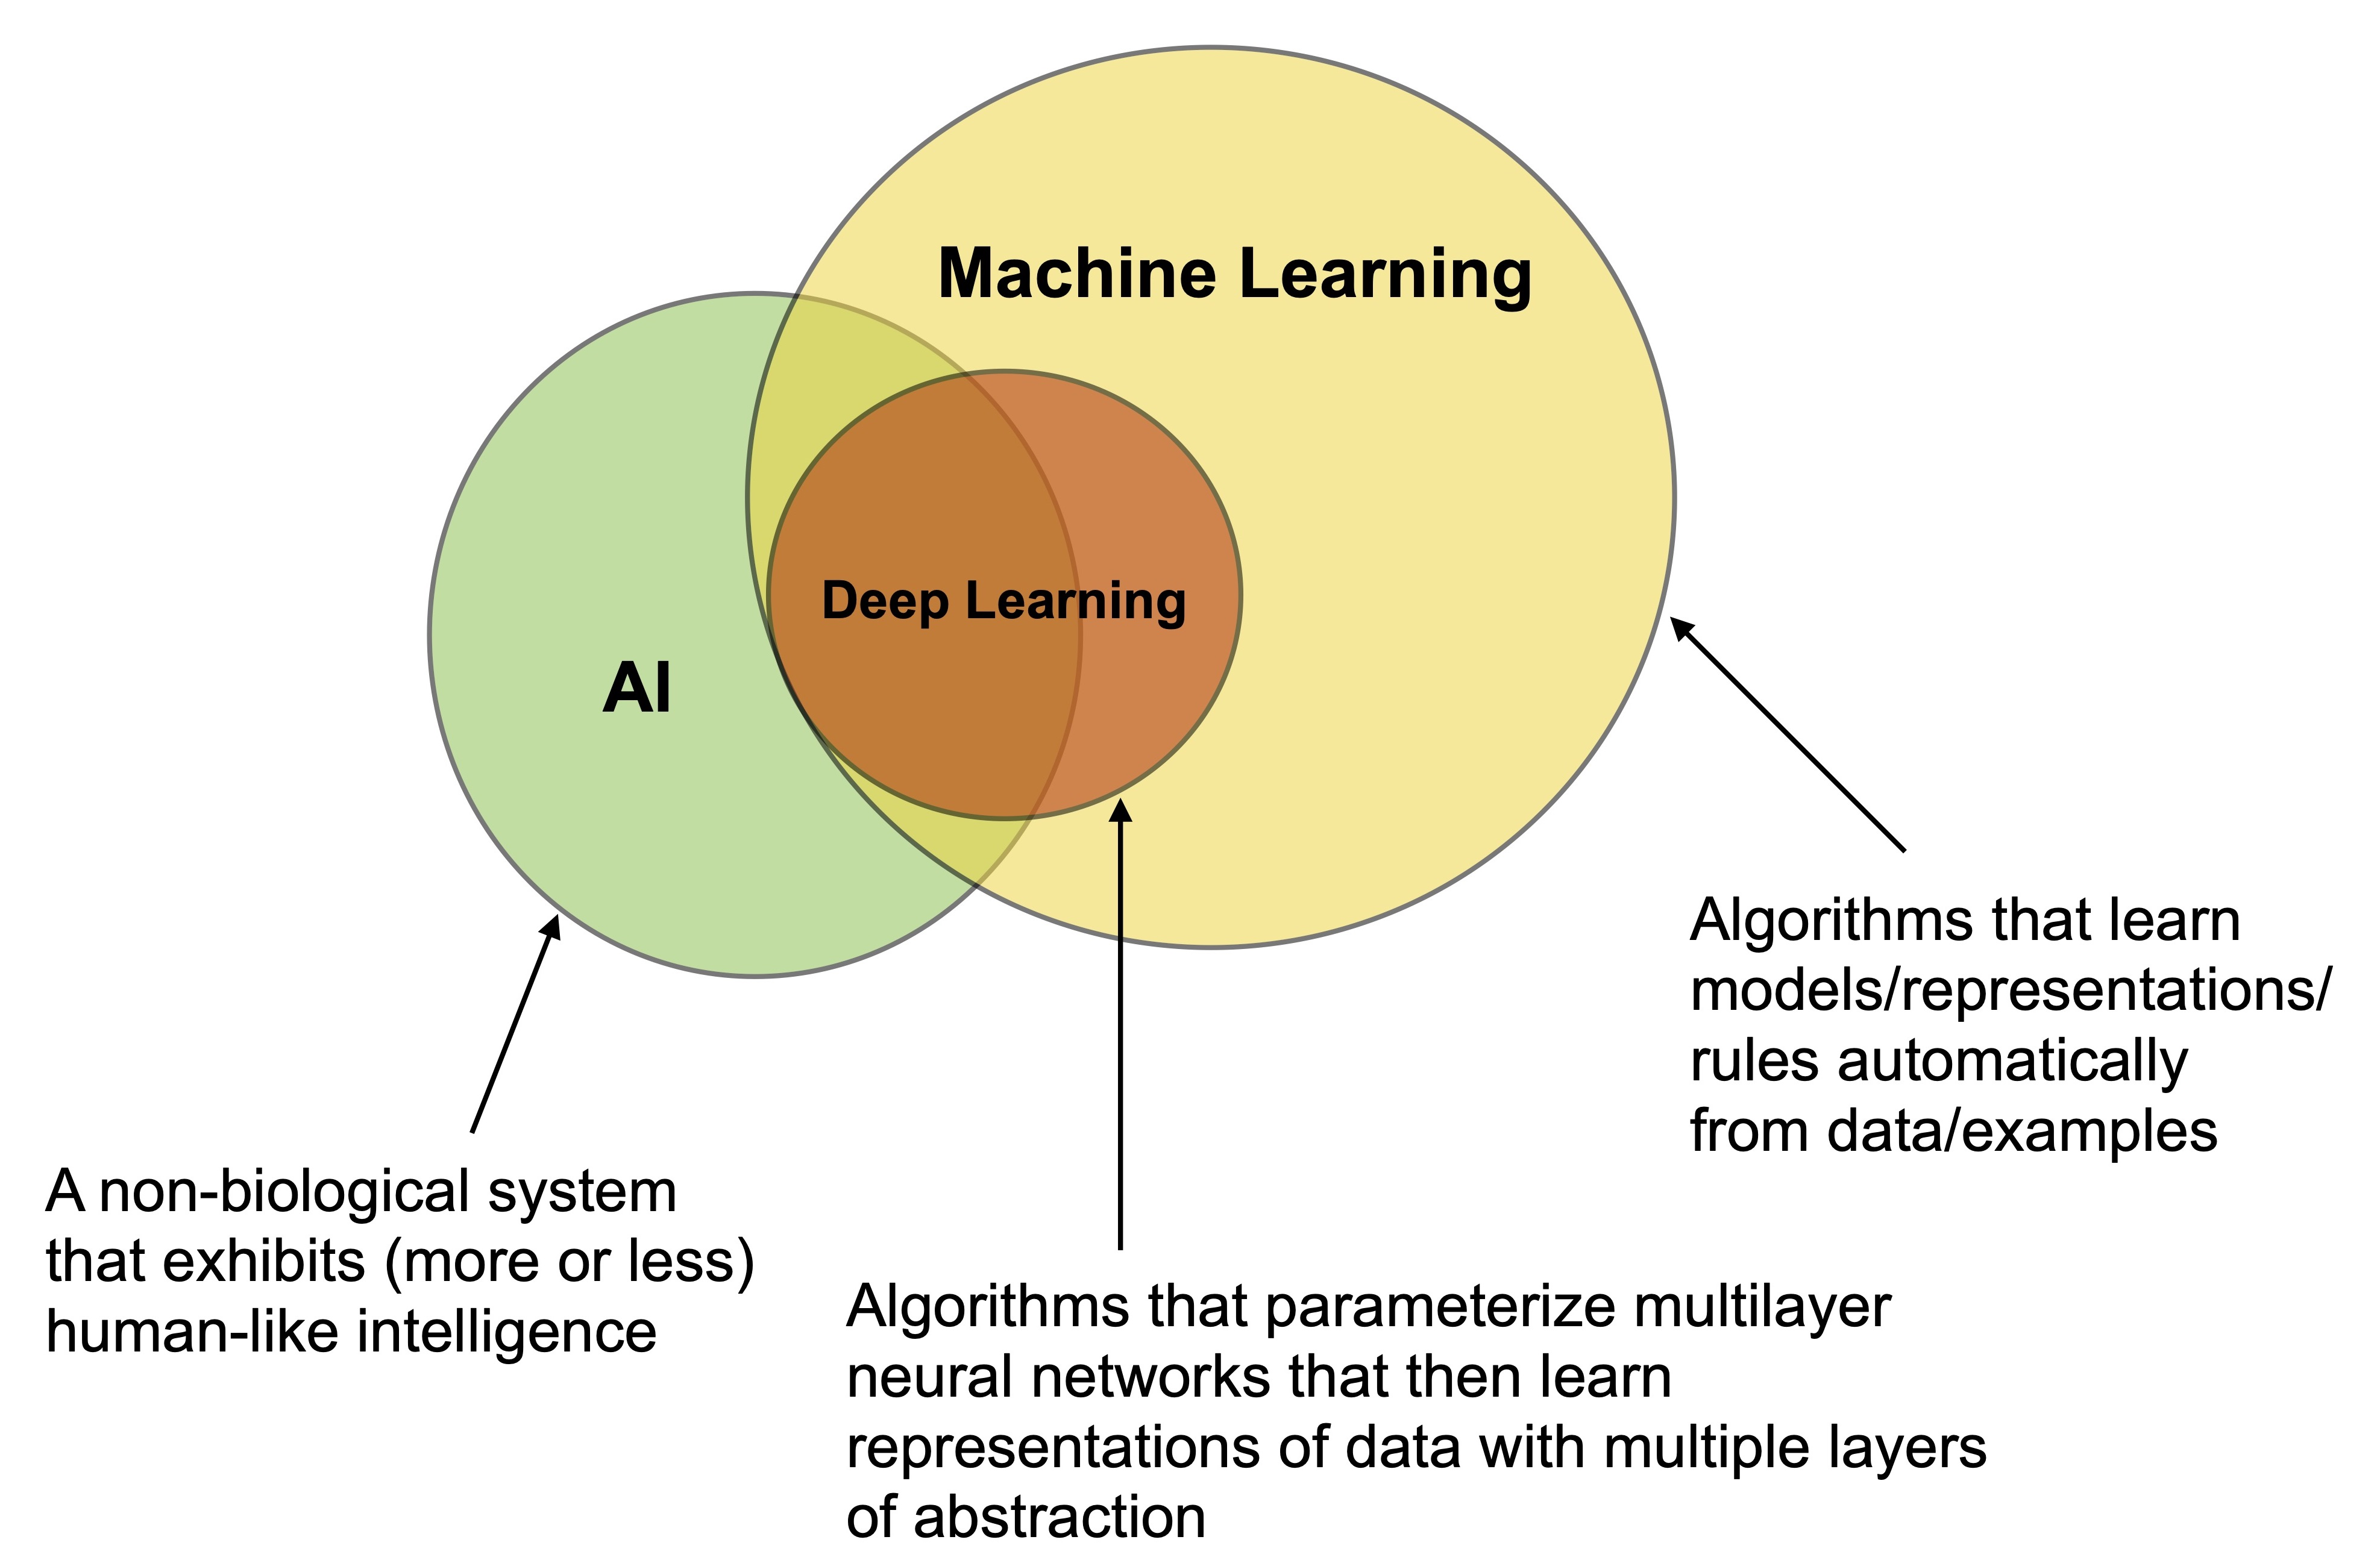
\includegraphics[width=13cm]{images/ai_ml_dnn_argue.jpeg}
        \caption[Overview of an alternative structure for \gls{ai}, \gls{ml}, and deep learning. This structure argues that AI is the quest for developing non-biological systems with human-like intelligence and can be achieved with methods that do not use machine learning or deep learning, like symbolic representations in a shallow architecture.]{Overview of an alternative structure for \gls{ai}, \gls{ml}, and deep learning. This structure argues that AI is the quest for developing non-biological systems with human-like intelligence and can be achieved with methods that do not use machine learning or deep learning, like symbolic representations in a shallow architecture. This representation is not de facto and will not be used in this thesis. Image credit: Raschka \cite{raschkaChapterIntroductionMachine0000}}
        \label{fig:ai_ml_dnn_argue}
    \end{figure} 

    \begin{figure}[htb]
        \centering
        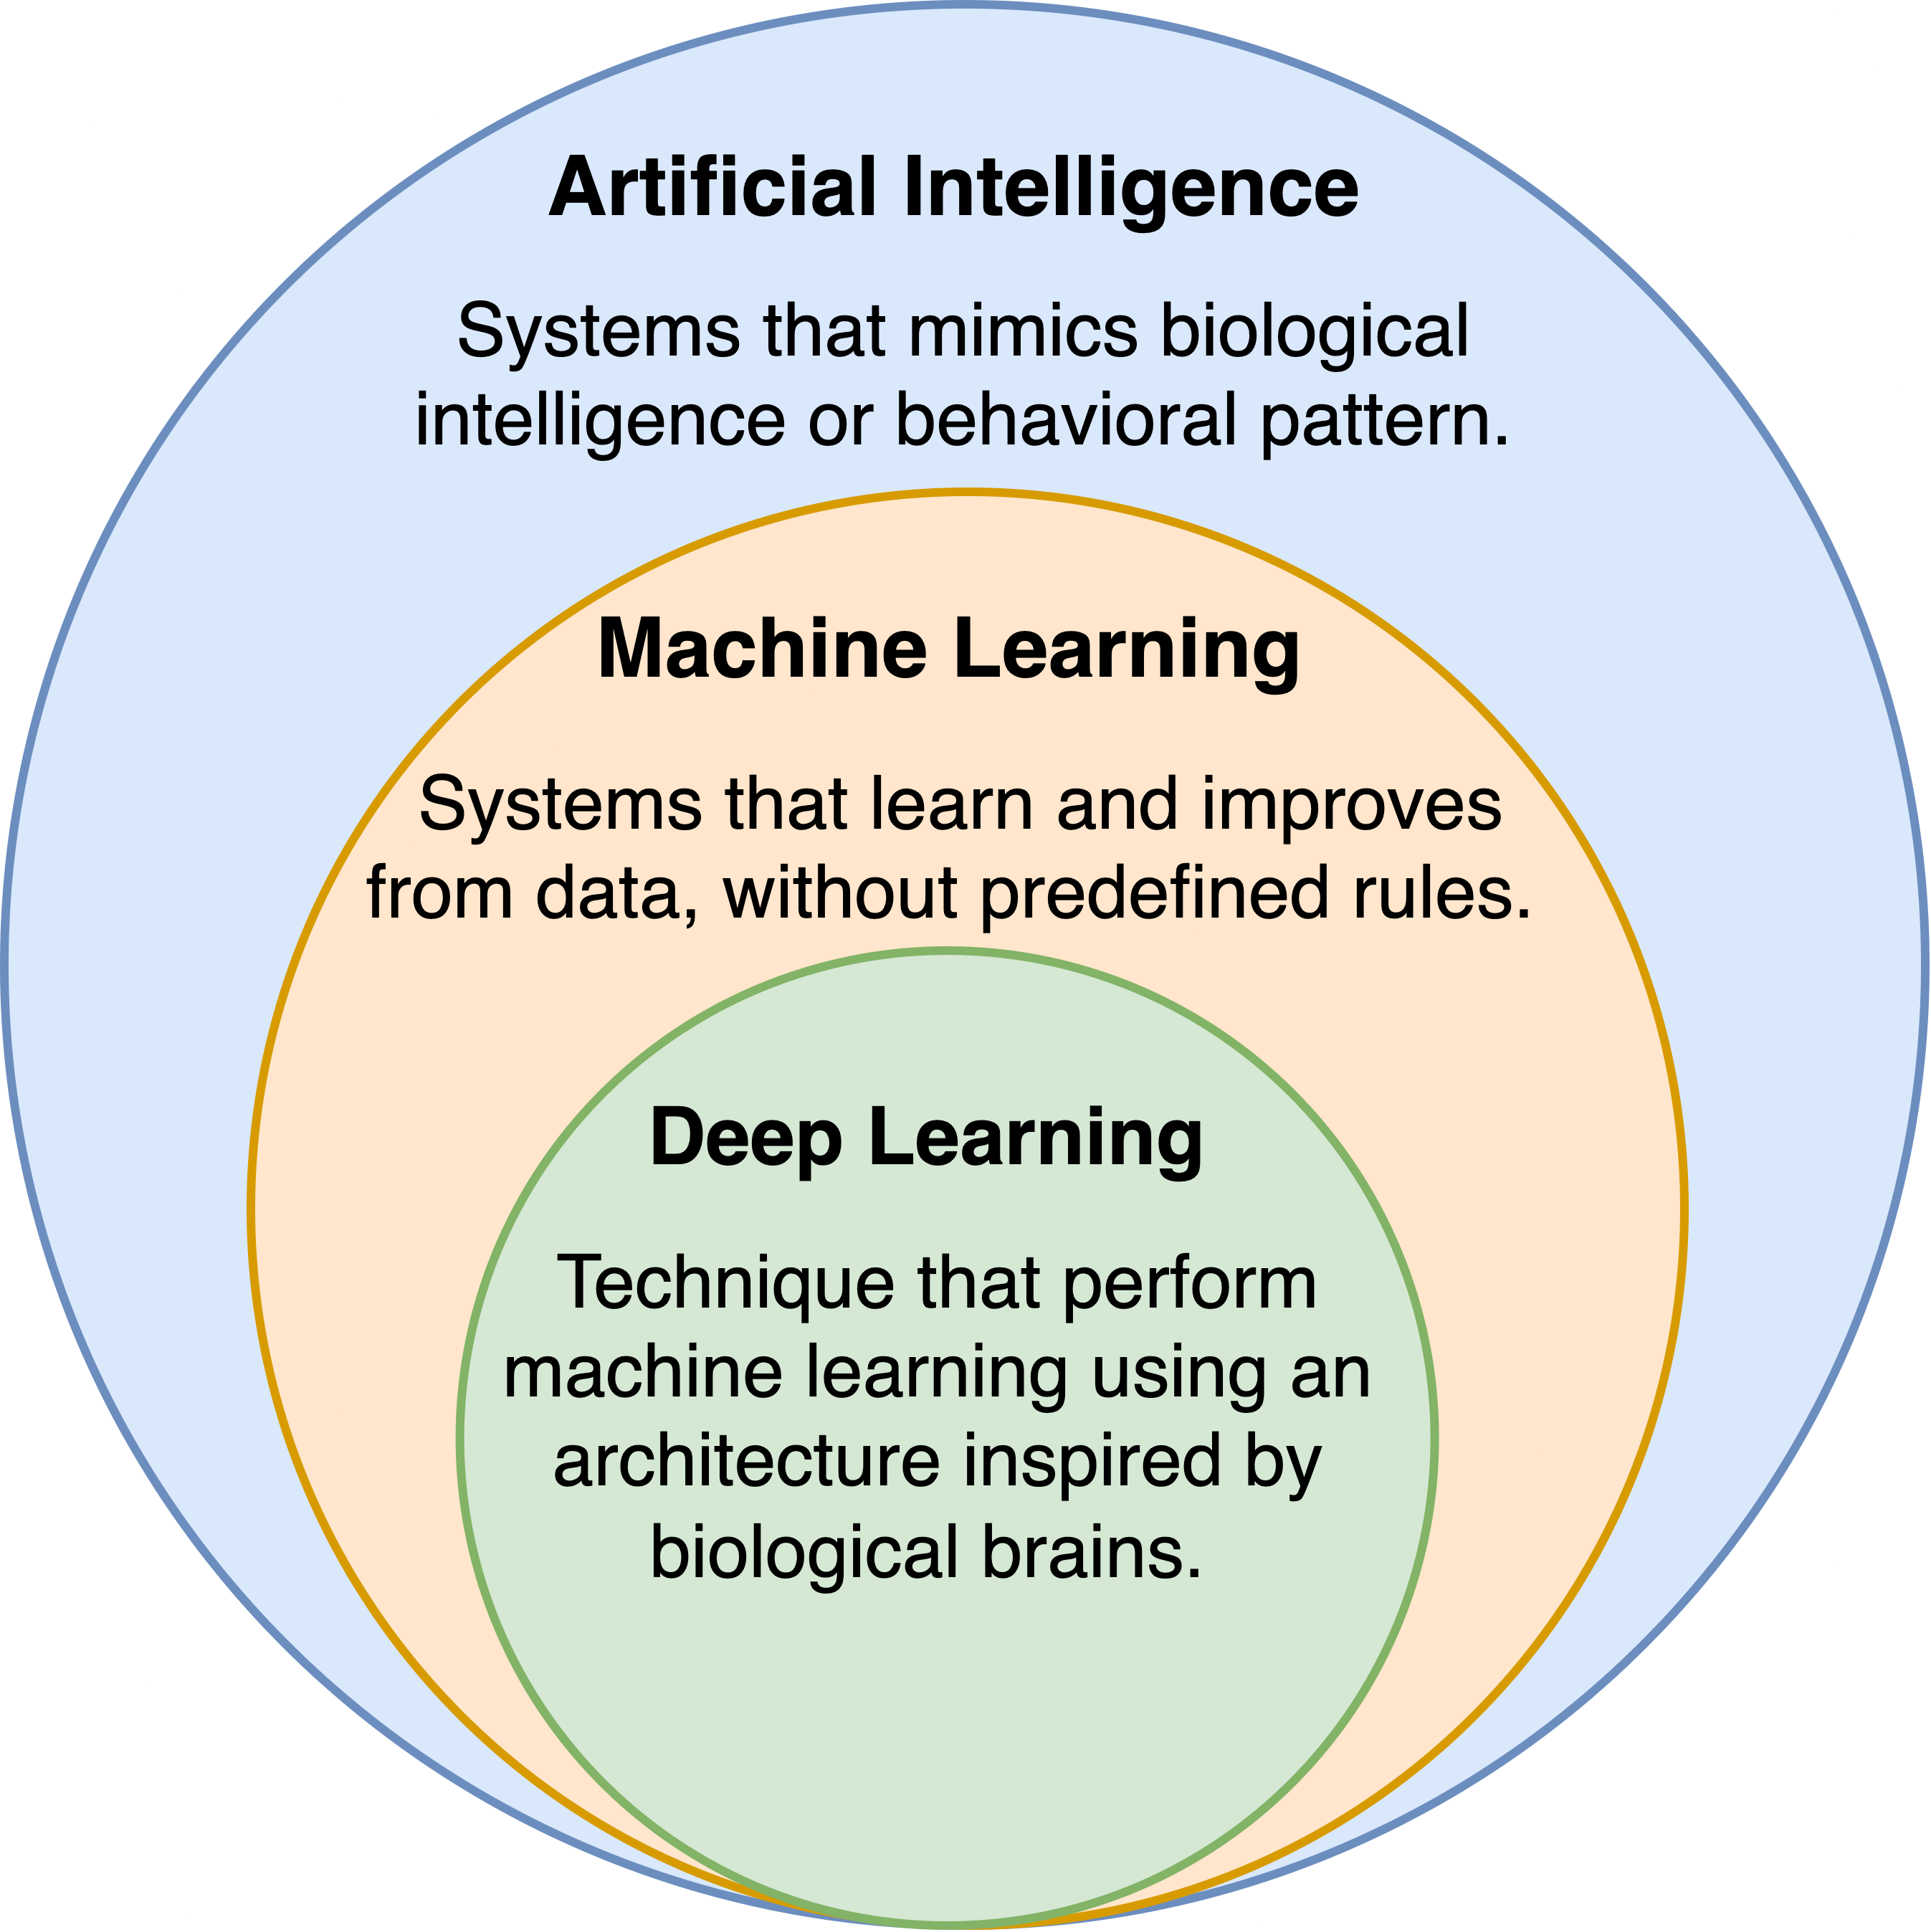
\includegraphics[width=8cm]{images/ai_ml_dnn.png}
        \caption{Overview of the structure between artificial intelligence, machine learning, and deep learning. This is the structure used in this thesis.}
        \label{fig:ai_ml_dnn}
    \end{figure} 

    Machine learning is often divided into three sub-fields, which will be discussed and explained in this sub-section, explaining how they work and the circumstances in which each sub-field can be used to advantage, as well as the challenges each branch faces are highlighted.

        \subsubsection{Supervised Learning}

        The first category within machine learning is known as supervised learning. This method is conceptually similar to using flashcards for memorization.
        The participant draws a card and reads the question while keeping the answer hidden. Only after the question has been answered by the participant can the correct answer be revealed. This is the same approach used in supervised learning.
        
        
        In supervised learning, a dataset with pre-labeled examples, also known as a fully labeled dataset, is used to train algorithms to predict labeling for unlabeled input data. This is typically accomplished by training on a larger dataset with labels for each input, passing the input through a network, and using the label to inform the algorithm what the input data should be labeled as. In this way, the method learns the connection between the input and the correct label. The method learns these correlations by adjusting the weights within the network to produce a result that is as close as possible to the true label.
        
        Since the ground truth label is known for each entry in the dataset, the model's output is compared to this ground truth label, and the accuracy of the closeness between these two is measured using a loss function. Weights are adjusted using backpropagation to minimize this loss, and training continues until the weights are appropriately adjusted to achieve a loss that is satisfactorily low. These weights are then used later when testing real-world inputs, for which ground truth is often unavailable, and needs to be estimated.
        
        Within supervised learning, there are two main subcategories: classification and regression. 
        
        Classification is a method used when the output variable belongs to a category, such as a color or an object, or to indicate the probability that an input belongs to one or more categories. Classification either predicts categorical class labels or classifies data by building a model. A typical classification method can be used to sort emails into spam or not spam or to identify the bird species in an image. Classification models can include methods such as neural networks, \gls{svm}, \gls{knn} \cite{fixDiscriminatoryAnalysisNonparametric1989, coverNearestNeighborPattern1967}, random forest, decision trees, one-vs-rest, and naive Bayes. Section \ref{sec:2_background_theory_deep_learning_and_neural_networks} will go into more detail about neural networks, as this is a very central method of machine learning and is relevant to this task.
        
        The second approach within supervised learning is called regression. This method is used when the output should be a real or continuous value. Regression is used to find the correlation between dependent and independent variables. Within regression, there are many different models, such as linear regression, logistic regression, and polynomial regression. It is common to use hyperplanes that fit the available data. Regression is often used to make forecasts based on past data, e.g. to estimate real estate prices for an area or salary growth.


        \subsubsection{Unsupervised Learning}

        Unsupervised learning is a technique that uses raw data from a given dataset to identify patterns and relationships in unlabeled data, facilitating the grouping of each item into appropriate clusters. The essence of this approach is that it can autonomously analyze and group data without requiring human intervention to pre-label the data. Therefore, it is well suited for use in data analysis, image recognition, and image segmentation.
        
        The main grouping models used in unsupervised learning are clustering, association, and dimension reduction. Clustering aims to divide raw data into groups or clusters based on similar characteristics. An example of a cluster split is shown in Figure ??, demonstrated by the \gls{knn} method. Association rules, on the other hand, are a rule-based approach that attempts to uncover relationships between variables in a dataset. These associations can be used in recommendation models, where companies can identify correlations between customers who purchase different items and use this knowledge to suggest similar products to new customers.
        
        Dimensionality reduction is a technique for reducing the number of dimensions in a dataset. 
        Although many methods benefit from additional data, this is not always the case. Data can often contain insignificant variables or mostly noise, making model training ineffective and reducing the size of the dataset. This technique can be used when creating a dataset and for visualizing and analyzing high-quality data. When reducing the dimensions of a dataset, the goal is to reduce the number of learnable parameters while maintaining the integrity of the data being processed. Well-known methods for dimension reduction are \gls{pca} and \gls{svd}. More recently, good results have been obtained with deep neural network-derived autoencoders. Autoencoders can compress data fed to them and produce a representation or encoding that retains much of the underlying data but is the dimensions are significantly reduced.
        To retrieve this data after encoding, a decoder is required to reconstruct the data. An autoencoder with an encoder and decoder is depicted in Figure ??.
        
        Unsupervised learning has proven useful in computer vision, where it can aid in object recognition, detection, and segmentation, such as in medical datasets. By allowing correlations to be identified and grouped into clusters based on features or traits, unsupervised ML can also be used for anomaly detection, where it can flag atypical data. This method is also often used in recommendation engines, such as those found in online stores, streaming services, or social media.


        \subsubsection{Semi-Supervised Learning and Hybrids}

        % https://en.wikipedia.org/wiki/Semi-Supervised_Learning#Semi-supervised_learning
        % https://en.wikipedia.org/wiki/Active_learning_(machine_learning)
        % https://ai.stanford.edu/blog/weak-supervision/
        % https://medium.com/geekculture/weak-supervision-and-active-learning-352fe8dc7df8
        % https://snorkel.ai/weak-supervision/
        % https://www.youtube.com/watch?v=SS9fvo8mR9Y
        % https://www.youtube.com/watch?v=-cc2RYF37zE

        Supervised learning is often more accurate than unsupervised learning as it can learn from the knowledge provided by humans in the form of labeled data. This approach can also avoid computational complexity since the model does not need to train on irrelevant features for the specific task. However, the downside of supervised learning is that it requires significant human effort beforehand, which can be time-consuming and costly, particularly when domain experts are required.

        A hybrid solution that aims to leverage the best of both supervised and unsupervised learning is known as semi-supervised learning. In technique pre-labels, only some parts of the input data are used for training. This approach can be beneficial when there is too much data to label, either because the dataset is large or the cost of labeling is high. Semi-supervised learning typically assumes that data points that are close together in feature space share labels or have an underlying correlation factor that is in a lower dimension (Manifold hypothesis/assumption). Methods using semi-supervised learning often achieve higher accuracy than those using only supervised or unsupervised approaches separately.
        
        Other approaches such as active learning and weak supervision are often used when a fully labeled dataset is not available for training. Active learning is a process in which a model can select input data about which it is unsure and ask a human or other expert for the correct answer. Such methods can be used to label large datasets, for example with Amazon Mechanical Turk. Samples are selected using a model that attempts to ask for samples believed to have the highest value for further classification. This can be achieved by first asking an expert for a sample of random samples and fitting the model to get a decision boundary that separates the classes. After that, the model can iteratively identify examples that are of high importance because they are near or on this decision boundary for the classification assessments and these are the most uncertain examples. Then the boundary is adjusted again and the process is repeated until a boundary is obtained that satisfactorily separates the data.
        
        Weak supervision is a method that can be applied in situations where it is preferable to have a large number of sufficiently accurate examples rather than a smaller number that are completely correct. This approach is often implemented by defining some rules or a knowledge base in advance, which helps the model estimate the probability that an example belongs to a certain category. Weak supervision is often used in conjunction with transfer learning, which involves transferring knowledge from one area to another. Transfer learning has shown promising results because generalizable data can often be transferred, eliminating the need to learn from scratch. Transfer learning can be combined with other methods, e.g. supervised learning.
    
    \subsection{Deep learning and Neural Networks} \label{sec:2_background_theory_deep_learning_and_neural_networks}
    Neural networks, also known as \glspl{ann}, are an ML method inspired by how the biological brain processes information and learns. Essentially, \glspl{ann} approach the goal of extracting information and constructing knowledge by forming a network of artificial neurons that can process input data. These artificial neurons, also called perceptrons, are the building blocks of the neural network and are likewise inspired by biological neurons. In this representation, the inputs to the artificial neuron are synapses on the dendrites, the activation function is inspired by the axon hillock, and the output from the artificial neuron is the biological axon.
    
    The artificial neurons process data by weighting the input data, together with a predetermined bias before passing it through an activation function, such as a sigmoid or ReLu, that produces the neuron's output. When the output of the activation function exceeds a certain threshold, the neuron is activated and sends data to the next layer. If the output does not exceed the threshold, no further data is sent.
    
    This processing step of a perceptron can be viewed as a linear regression, as in shown formula ?. However, unlike linear regression, perceptrons in \glspl{ann} are connected in a network, so changes in weights cascade to the next level of perceptrons. A single layered neural network can therefore be seen as a logistic regression function.
    
   \glspl{ann}, often called multi-layer perceptron (MLP), are the cornerstone of deep learning, which refers to \glspl{ann} with more than three layers. The smallest deep network, therefore, has an input layer, two hidden layers in the middle, and an output layer. These middle processing layers are called the hidden layer because it is hidden from the outside, which the input and output layers are not. An example of such a network with 2 hidden layers is shown in Figure \ref{fig:deep_network} to see. 


    \begin{figure}[htb]
        \centering
        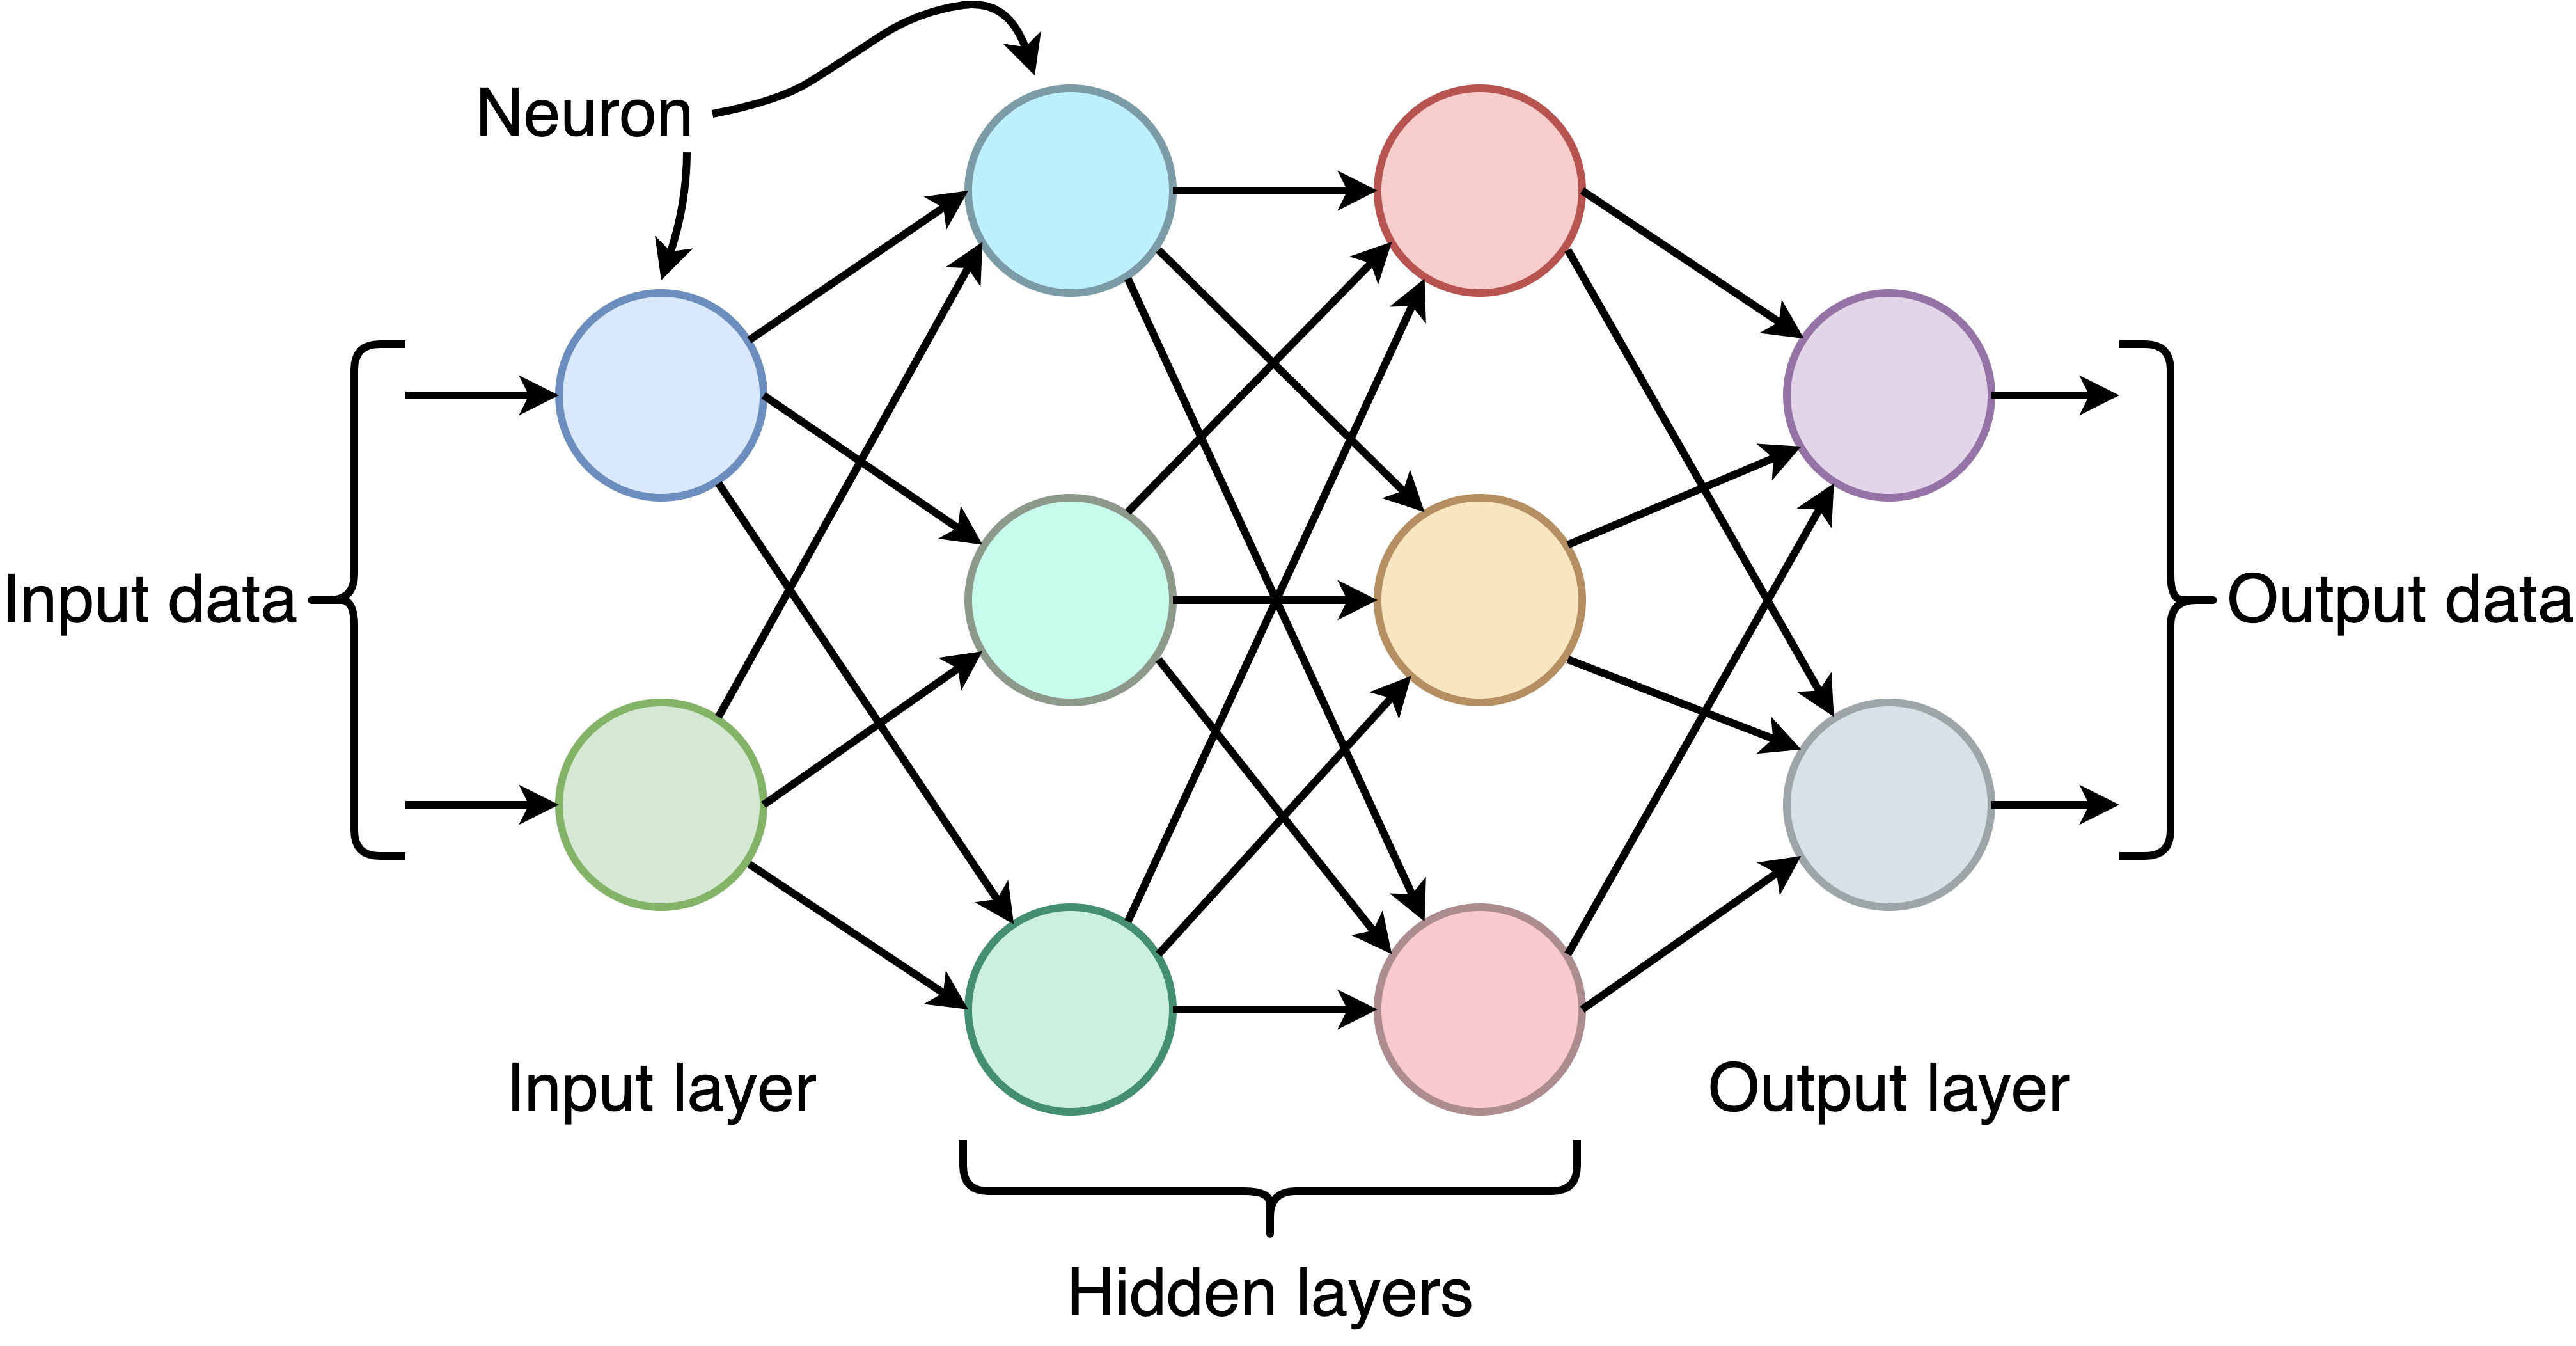
\includegraphics[width=12cm]{images/deep_neural_network.png}
        \caption{A fully connected deep artificial neural network with two hidden layers and two input and output neurons.}
        \label{fig:deep_network}
    \end{figure}

   
    
    Most \glspl{ann} are feedforward, meaning that data is entered on one side, passed through the network, and produces a result on the other end. They are often trained using backpropagation, where the network output is compared to the ground truth and the difference between the guess and the ground truth is used to adjust the network weights to minimize the difference. The backpropagation technique is also inspired by biological backpropagation, which occurs when a neuron generates an action potential that sends a voltage spike back to the dendrites. There are also other methods proposed instead of feed-forward, such as the recently proposed forward-forward algorithm by Hinton \cite{hintonForwardForwardAlgorithmPreliminary2022}.
    
    Deep neural networks have achieved great success, mainly due to their ability to learn from both structured and unstructured data, which allows them to learn and generalize knowledge given sufficient and high-quality data. Before computing power allowed the use of deep networks, hand-made feature extractors were commonly used, using human-predefined features such as texture, shape, and color for object recognition tasks. However, when deep learning was first used in the \gls{imagenet} competition \cite{russakovskyImageNetLargeScale2015}, a competition to identify objects from ImageNet \cite{russakovskyImageNetLargeScale2015}, as shown in Figure \ref{fig:imagenet_results_graph}. In this figure, we see the methods that won the competition in different years. It is clear that deep learning made significant strides in 2012 with AlexNet, which was proposed by Krizhevsky et al. \cite{krizhevskyImageNetClassificationDeep2017}, and these methods have continued to improve significantly since then, largely thanks to improved methods and hardware. In 2015, deep learning even surpassed the human ability to classify images in ImageNet \cite{heDeepResidualLearning2015, heDelvingDeepRectifiers2015}.
    
    \begin{figure}[htb]
        \centering
        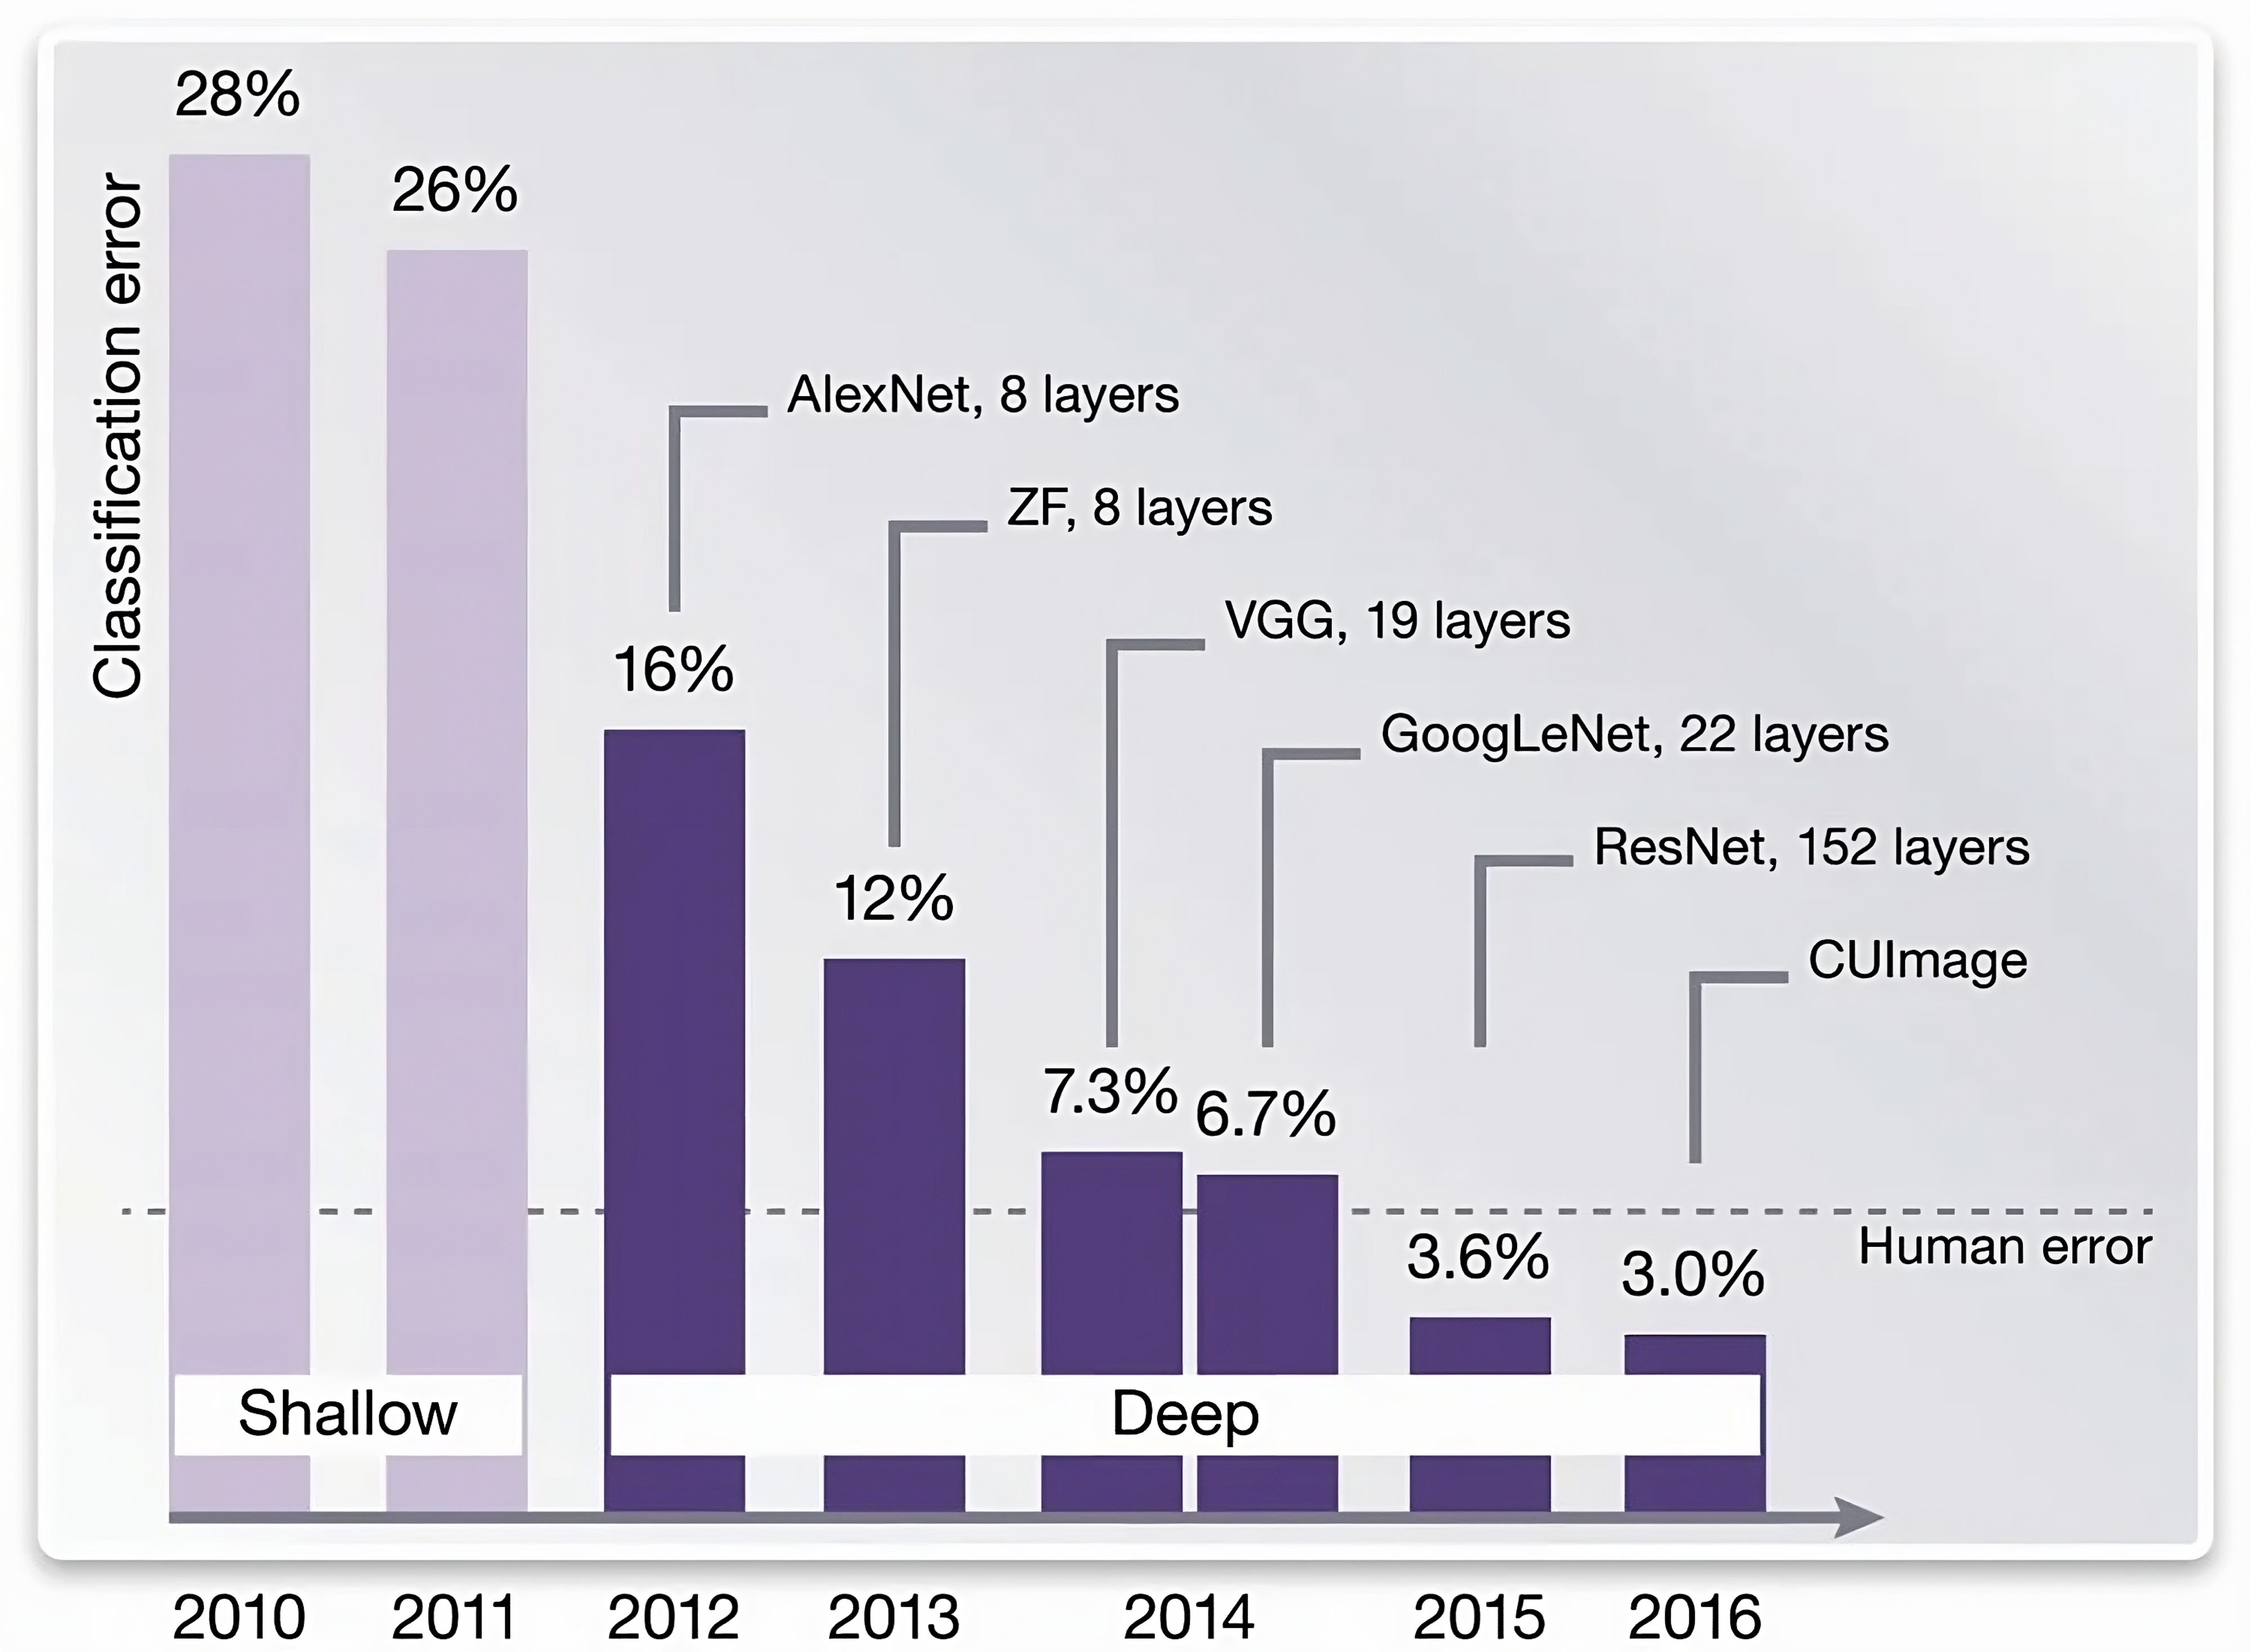
\includegraphics[width=12cm]{images/imagenet_results_graph.jpeg}
        \caption[Overview of the ImageNet competition winners from 2010 to 2016.]{Overview of the ImageNet competition winners from 2010 to 2016. The figure shows how deep networks have significantly improved the networks' ability to guess the right label for the images in the ImageNet dataset. In 2015, the deep network ResNet \cite{heDeepResidualLearning2015} surpassed the average human ability to correctly label these images. \\
        Image credit: Gordon Cooper \cite{cooperSoftwareFrameworkRequirements2017}.}
        \label{fig:imagenet_results_graph}
    \end{figure}


    
    \subsection{Convolutional Neural Networks}

    % Intro to CNNs
    Inspired by biology alongside regular neural networks, the computer vision method called \glspl{cnn} are designed to mimic the way the visual cortex in the brain processes visual information. \gls{cnn} builds on the idea and technique of neural networks and adds at least one convolutional layer. A convolutional layer allows information about neighboring entities to be obtained from the previous layer. The method has proven particularly effective in computer vision to process and analyze images and video because it can gather context from nearby areas around which the convolution is centered. This can help the method extract contextual and semantic relationships that would otherwise have been lost.

    % Intro to convolution layer
    The convolution layer works by scanning small filters across the input image, computing dot products between the filter and the image pixels at each location, and creating a feature map. A convolution layer can be thought of as a flashlight beam aimed at an image. Because of the beam of light, the viewer can see areas of the image that are in the perimeter of the area at which the center of the beam is directed. As the beam of light moves across the image, the viewer gets a fuller understanding of what is in the image. An illustration of a convolution is shown in Figure ?? shown.

    % Short history and advantage.
    The convolutional neural network was first proposed by ??? in ?? and has since had a huge importance in making machines interpret images and videos. A major advantage of a convolutional layer is that it can compress information while preserving information and the context around the retrieved information. A very common \gls{cnn} architecture is shown in Figure ??? to see. Also seen in the figure is that a typical \gls{cnn} has a fully connected neural network. The reason that a \gls{cnn} often uses fully connected layers, unlike a normal neural network, is because of the condensation of information with surrounding information, allowing for a network that can take advantage of using a lot of parameters without overfitting.  
    
    The convolution layers can be applied to an input image as a series of filters, producing a series of feature maps that emphasize different aspects of the image. These filters have weights that are learned and adjusted during training and are able to recognize different types of patterns of increasing complexity and abstraction from the input image. The training process is similar to regular neural networks and typically updates weights using backpropagation to minimize the loss function and improve the accuracy of the network on the training set. The first layers, closest to the input image, generally recognize low-level features such as edges, lines, corners, texture, and color. As the input information is processed by the convolutional layers, more complex features can be detected that build an abstraction on the information extracted from earlier layers. Convolution layers farther from the image can recognize more high-level features such as shapes, objects, and scenes. Overall, the convolutional layers allow the features of the input image to be analyzed hierarchically, with the early layers capturing low-level features and the later layers capturing high-level features.
    
    % More in depth achitecturea, with pooling layers.
    \glspl{cnn} are typically designed with multiple layers, like deep neural networks, and the last layers are typically fully connected. The fully connected layers take the output of the convolution layers, which are a set of feature maps, and convert them into a single vector of class scores that represent the probability that the input image belongs to each of the possible classes. The main function of pooling layers in \glspl{cnn} is to reduce the spatial dimensions of the feature maps generated by convolutional layers while preserving the most salient features of the input image. Pooling layers operate on small regions (e.g. 2x2 or 3x3) of the feature maps generated by the previous convolution layers and reduce their size by applying a pooling function such as max pooling or average pooling, on each region. Max pooling selects the maximum value within each region as the representative value, while average pooling calculates the mean of the region. These operations effectively downsample the feature maps and help reduce the network's sensitivity to small spatial translations and variations in the input. Pooling layers can be inserted after one or more convolutional layers in a \gls{cnn}, and their hyperparameters, such as the size of the pooling area and the stride (i.e. the amount of movement of the pooling window) can be tuned to control the amount of downsampling and the size of the resulting feature maps.
    
    Additionally, pooling layers can help prevent network overfitting by reducing the number of parameters and the computation time required for training. The role of pooling layers in \glspl{cnn} is not only limited to downsampling, but they can also help to capture translation invariance, i.e. the property that the learned features are invariant to small translations in the input. This is because the Max or Average operation selects the most prominent feature in a given region, regardless of its exact position within that region. This property allows the network to collect more general relationships in the input data, providing a more general understanding of the network. The overall benefits of pooling layers lie in reducing the spatial dimensions of feature maps while preserving their salient features, resulting in more efficient and robust image analysis.
    
    % Summary
    Overall, the different layers of a \gls{cnn} work together to extract and classify features in images and videos. This makes \glspl{cnn} particularly effective for tasks such as image classification, object detection, and semantic segmentation, where detecting and locating different features of an image is critical for accurate performance. \glspl{cnn} have proven extremely effective in image classification tasks, outperforming other types of neural networks and traditional machine learning algorithms. They have been used in a variety of applications, including object recognition, facial recognition, and medical image analysis. With the development of larger and more complex networks and the availability of powerful hardware and software, \glspl{cnn} continue to remain an active area of research and development in the field of machine learning.


\section{Image Captioning}

    Image captioning is a field of research where the objective is to generate textual descriptions from the content of an image. This process uses both computer vision and \gls{nlp} to gather information from images and give a text that describes or analyzes the content of the image. Image captioning is therefore a multimodal method that has excelled together with the advancements in both computer vision, helped greatly by \glspl{cnn} and language models. The motivation for developing this field of research is that its advancements can be utilized in many applications. Some applications where image captioning can contribute are in improving accessibility for the visually impaired, enhancing search and retrieval systems, assisting in image and video indexing, and making models that can use the combined information in both language and vision to gather information. 

    Image captioning methods involves typically today techniques from deep learning, with \glspl{cnn} to extract image features and \glspl{rnn}, typically \glspl{lstm}, to use these extracted image features to generate captions. An advantage of the multimodal nature of image captioning methods is that the \gls{cnn} are able to capture spatial features within a given image, while the \gls{rnn} can structure this information, using temporal dynamics and syntaxes in language to make a description that is true to the image. 


    \subsection{Attention Mechanisms}
    % Attention is all you need
    Recent advances in image captioning have seen the use of attention mechanisms, both in the vision and language modalities. The use of attention mechanisms has allowed the model to selectively focus on different parts of the image when generating captions. By selectively paying attention to different areas of the image, the model is able to capture the fine-grained details needed to generate accurate and descriptive captions. This has resulted in a significant improvement in the quality of captions, where attention-based methods often outperform traditional non-attention-based techniques. 
    
    The attention technique is inspired by nature and is designed to draw inspiration from cognitive attention. The main advantage is that attention allows the method to enhance some parts of the input data while giving a lower priority to other, less important parts. One goal is to use attention to learn which parts of the data that is most important in the context and prioritize these parts.  


    % One attention method that has made huge advancements is the Transformer architecture proposed by Vaswani et al. The Transformer differs from a traditional network in that it entirely dispenses recurrence and convolutions. Instead, it is solely based on the attention mechanism, using self-attention and point-wise, fully connected layers for both the encoder and decoder of the architecture. 

    Attention-like mechanisms have been part of the research field of machine learning since the 1990s. In the beginning, it was introduced under names like sigma pi units, multiplicative modules, and hyper-networks. The flexibility of attention-based techniques comes from their ability to learn which parts of the input data are most important in context. The soft attention method can change the model's focus during runtime, which can have a major advantage compared to non-attention models, which remain unchanged during inference. The ability to adaptively prioritize input data has popularized attention-based models in natural language processing, multimodal, and multisensory computing. Some influential methods that use attention are \glspl{lstm}, Transformers, and Perceivers \cite{hochreiterLongShorttermMemory1997, vaswaniAttentionAllYou2017, jaeglePerceiverGeneralPerception2021}. The use of transformers and attention mechanisms have made it possible to make large language models, such as \gls{bert}, \gls{bart}, and \gls{gpt} \cite{devlinBERTPretrainingDeep2019, lewisBARTDenoisingSequencetoSequence2019,, radfordImprovingLanguageUnderstanding2018, radfordLanguageModelsAre2019, brownLanguageModelsAre2020, openaiGPT4TechnicalReport2023}. 
    
    
    In the language part of the model, the attention mechanisms can also be used to selectively focus on a different part of the features extracted from the image and can therefore generate the textual context that is most relevant to correctly identify. This way the model can describe the most important ones in natural language parts of the picture or video. Some recent models have moved from cnn architectures to extract image features and solely rely on attention mechanisms to gather relevant information in the visual context. Some recent models have moved from CNN architectures to extract image features and solely rely on attention mechanisms to gather relevant information in the image context. Some of these models are \gls{vit}, alongside versions of \gls{bert} that incorporate vision \cite{leiLessMoreClipBERT2021, liVisualBERTSimplePerformant2019, suVLBERTPretrainingGeneric2020}. % An image is worth 16x16 words: Transformers for image recognition at scale, ViBert 
    
    During training, attention weights are most commonly learned through backpropagation and gradient descent, and the weights are used to give relevance scores to different words in context for being the next word in the text sequence. Attention can be derived in a number of ways, notably global vs local and soft vs hard. Global vs. local attention refers to different ways of weighting input features, where a global process weights all input features equally without prioritizing specific parts, and each input feature is considered when computing the output.
    In contrast, local attention refers to a more selective process in which the input features are weighted differently and are therefore prioritized when computing the output. This prioritized subset is usually determined by a region or window around the previous output or target position, borrowing ideas from the way \glspl{cnn} retrieves surrounding data from an image.
    
    Soft and hard attention refers to the different methods of incorporating attention into a neural network. Soft attention is computed by a weighted average of the input features, with the weights learned during training and typically normalized to a value between 0 and 1. This weighting allows the model to consider multiple parts of the input at once, gathering information from a larger range. On the other hand, hard attention selects a particular input feature to take care of at each time step, effectively forcing the model to make a discrete decision. This can make the model less flexible but can excel in situations where the input is highly structured and can be easily segmented into distinct parts.


    
    \subsection{Image Classification}


    \subsection{Natural Language Processing}
    % Labeling / Captioning
    \subsection{Automatic Labeling}



\section{Visual Question Answering}
    % What is VQA

    % Why is VQA important and interesting
    

   

% Datasets
\section{Datasets}
    % ImageNet

    % MS COCO

    % Different VQA datasets
    
    % What is the VQA 2.0 dataset

     

    \subsection{Dataset Splitting} 


\section{Model evaluation}

    \subsection{Performance Metrics}


\section{Frameworks}